% !TEX root = ../main.tex
\chapter{Employ the Learned Deep Model}\label{ch:chapter5} % For referencing the chapter elsewhere, use \ref{Chapter1}
%
%%----------------------------------------------------------------------------------------
%
After obtaining the learned models which exhibit desired behavior, 
their integration into the reference software is carried out.
In this chapter, the time cost of the model prediction
is analyzed and optimizing methods are described.
After that we explain the details of the algorithm for integration.
In the end of the chapter the results of experiments 
are presented with discussions.

%3D Video applications are attracting more interests
%%----------------------------------------------------------------------------------------
%
\section{Analysis and Optimisation for Prediction Time}\label{sec:analysis-and-optimization}
% In C++ APIs from Tensorflow version 1.1, if we want to run the prediction,
% a unique session has to be initialized in which the predicting activities 
% take place.
% It is found that the session initialization is very time expensive.
It is intuitive to think in this way: 
every time when the encoder encounters a new block in the video frames,
the learned models are required to perform the prediction for that block.
However, after this idea has been implemented, it turns out the
time cost of the encoder with neural engine even gets much higher 
than the encoder without neural engine.
We found that the idea of one prediction for one block actually
introduces a problem that impedes the integration to work as expected:
a new session is initialized for a prediction, and the initialization
for a single session in Tensorflow C++ APIs actually is very time
expensive.
The other idea which is a better way would be a single 
session for a batch of blocks.

The time cost of session initialization has been investigated
and compared between the two ideas aforementioned.
The learned model for blocks of size \(8\times8\) is loaded 
to run predictions for blocks of size \(8\times8\) from one single
frame in one video sequence with the resolution to 
be \(1024\times768\).
Totally 12288 blocks to predict.
When compiling the executable binary of the encoder
powered by neural engine, it can be compiled 
against CPU or GPU when the compilation tool 
called Bazel~\parencite{RN200} is utilized.
Even more, with Bazel, the AVX and SSE4.2 can be employed to
accelerate the parallel computations in one instruction
at single moment in CPU\@.
They offer more efficient matrix computations
to CPU\@.
Six experiments have been conducted and the results
are shown in 
Table~\ref{tab:seesion-init-plain-cpu}.
% on page~\pageref{tab:seesion-init-plain-cpu}.

\begin{table}
    \caption{Time cost of session initialization for two ideas based on three sets of compiling configurations}
    \bigskip\label{tab:seesion-init-plain-cpu}
    \centering
    \begin{tabular}{c c c c c}
        \toprule
        \# & Idea & Plain CPU & AVX and SSE4.2 & AVX, SSE4.2 and GPU \\
        \midrule
        1 & initialize 1 session for 12288 blocks & 21.37s &15.56s&2.03s \\
        2 & initialize 12288 sessions for 12288 blocks & 47.81s &33.91s&55.26s\\
        \bottomrule
    \end{tabular}
\end{table}

Obviously the best way is to compile the 
executable binary against AVX, SSE4.2 and GPU, at the same
time use the idea of one session for multiple blocks.

\section{The Integration of the Learned Model}\label{sec:integration-of-learned-model}
We have integrated two learned models into 
\(HTM16.2\) which is the newest version of
the reference software of 3D-HEVC by the time this thesis
is written\@.
More specifically, ResNet engines have been integrated to 
\textbf{\textit{TAppEncoder}} in \(HTM16.2\) for depth map 
angular modes [2, 34] prediction and the DMM1 searching process.
Wedgelet slope is employed
to reduce the number of wedgelet candidates to be evaluated in DMM1 
searching process. 
Since top-15 is used, roughly half of the candidates are skipped
during the encoding time.

The details of the proposed fast depth coding algorithm is shown 
in Figure~\ref{fig:proposed-fast-depth-coding-algorithm}
on page~\pageref{fig:proposed-fast-depth-coding-algorithm}.
Initially, before the encoding of a depth map will start, 
its Luma pixel values are accessed by the learned models to
predict best modes for all the suitable blocks inside it.
We call it \textbf{Batch Prediction}.
Next, for each depth block of 
size \(8\times8\), \(16\times16\) and \(32\times32\), 
top 15 modes together with PLANAR, DC modes are added to 
a candidate list for Rough Mode Decision (RMD).
For blocks of other sizes, the original encoder workflow
is applied.
Then if mode 2 is inside the RMD list, mode 34
will be added to RMD list due to the reason that
it is of the same angle as mode 2.
Else if mode 2 is not inside the RMD list, 
mode 34 will not be added to RMD list.
Then Sum of Absolute Transform Difference (SATD)
is used to obtain the best 3 candidates for blocks
of size \(8\times8\) and \(16\times16\), 2 candidates
for blocks of size \(32\times32\).
After SATD, the best prediction of the block
is utilized to construct a range of slopes.
Denote the number of the top-1 mode from the model 
prediction as \(N_1\), a slope range will be constructed 
using the angular modes within \([N_1-7, N_1+7]\), where
the two boundaries are inclusive.
In the further step, when performing the DMM1 coarse
searching, the wedgelets which have the slopes out of the 
constructed slope range are excluded from 
View Synthesis Optimization (VSO) which is the
source of the computational complexity in the original
encoder.
The DMM1 refinement following the coarse search is unmodified.
In the end, the best mode for the
depth map to be coded in the encoding process will
be obtained.
This algorithm can reduce the wedgelets to be evaluated by 
roughly half.
Besides, as a bonus, the conventional intra 
angular mode decision for depth maps is also
accelerated using the same prediction from 
neural networks.
% First 

\begin{figure}
    \centering
    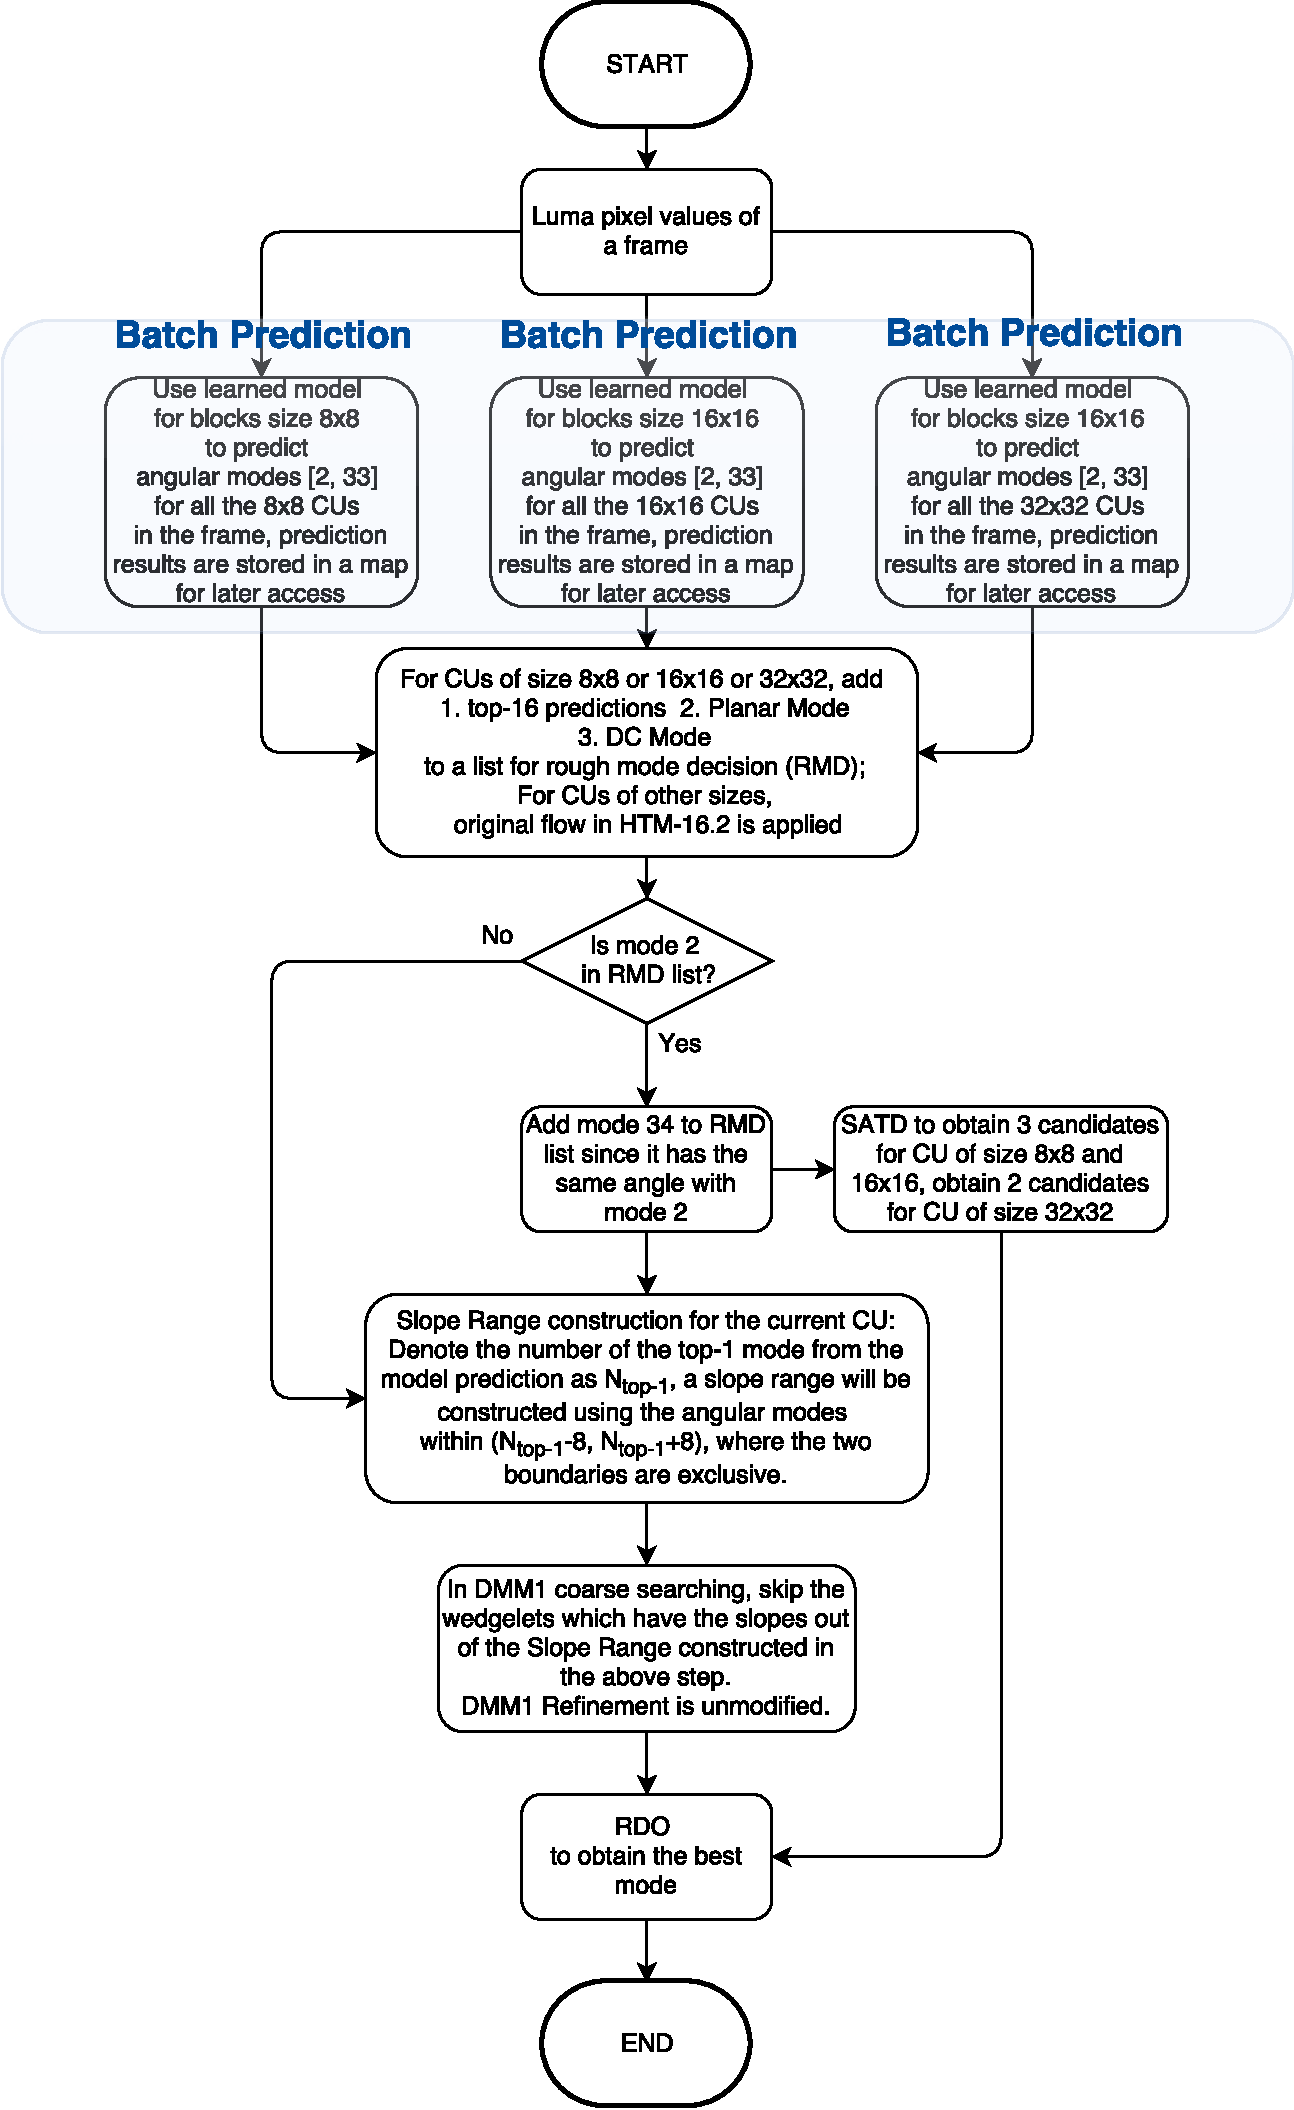
\includegraphics[height=0.92\textheight,keepaspectratio]{Figures/proposed-fast-depth-coding-algorithm}
    \caption[Flowchart for proposed fast depth coding 
    algorithm]{Flowchart for proposed fast depth coding 
    algorithm.}\label{fig:proposed-fast-depth-coding-algorithm}
\end{figure}

\section{Results of Experiments}\label{sec:simu-results}
The experiments are conducted on four video sequences shown in
Table~\ref{tab:data-for-experiments} on
page~\pageref{tab:data-for-experiments} to make sure every sample
that will be predicted has never been seen by the learned models.
Two metrics of \textbf{BD-BR} in~\parencite{RN234} and \textbf{BD-PSNR}
in~\parencite{RN235}
are used in the evaluations for the objective quality
of reconstructed videos.
\textbf{BD-BR} calculates the differences on average for
the RD curve of the synthesis views and the overall bitrate 
for all the frames in the video sequences.
\textbf{BD-PSNR} is employed to assess the subjective 
quality of synthesized views.
The common test condition defined
in~\parencite{common-test-condition}
is used.
All the frames from the four video sequences in experiments 
are encoded as I-Frames.
\begin{table}[!htbp]
    \caption{Video sequences used for experiments}
    \bigskip\label{tab:data-for-experiments}
    \centering
    \begin{tabular}{c c c c c}
        \toprule
        \# & Name of the Sequence & Resolution & Usage & Number of Frames\\
        \midrule
        1 & Newspaper & \(1024\times768\) & Simulation & 300\\
        2 & GhostTownFly & \(1920\times1088\) & Simulation & 250\\
        3 & PoznanHall2 & \(1920\times1088\) & Simulation & 200\\
        4 & Shark & \(1920\times1088\) & Simulation & 300\\
        \bottomrule
    \end{tabular}
\end{table}

Table~\ref{tab:ts-dmm}
% on page~\pageref{tab:ts-dmm}
shows the time saving for DMM1 wedgelet searching process together 
with the coding performance.
Table~\ref{tab:ts-total}
% on page~\pageref{tab:ts-total}
presents the time saving for total encoding and the coding performance.

\begin{table}[!htbp]
    \caption{Time saving for wedgelet searching and coding performance of proposed method}
    \bigskip\label{tab:ts-dmm}
    \centering
    \begin{tabular}{c c c c c c c}
        \toprule
         & \multicolumn{4}{c}{Time saving for DMM1} & & \\\cline{2-5}
        Sequences & QP34 & QP39 & QP42 & QP45 & BD-BR & BD-PSNR \\
        \midrule
        Newspaper       & 63.76 & 64.94 & 71.98 & 74.14 & 0.98\% & -0.02dB \\
        PoznanHall2    & 71.08 & 71.08 & 66.36 & 71.27 & 1.64\% & -0.05dB \\
        GhostTownFly       & 62.00 & 56.20 & 51.60 & 58.87 & 0.65\% & -0.02dB \\
        Shark           & 63.55 & 58.66 & 63.26 & 63.34 & 1.04\% & -0.03dB \\
    \end{tabular}
\end{table}

\begin{table}[!htbp]
    % \begin{table}[!htbp]
    \caption{Time saving for total encoding and coding performance of proposed method}
    \bigskip\label{tab:ts-total}
    \centering
    % \resizebox{\textwidth}{!}
    % {
    \begin{tabular}{c c c c c c c}
        \toprule
         & \multicolumn{4}{c}{Time saving for total encoding} & & \\\cline{2-5}
        Sequences & QP34 & QP39 & QP42 & QP45 & BD-BR & BD-PSNR \\
        \midrule
        Newspaper       & 27.33 & 27.20 & 27.78 & 27.38 & 0.98\% & -0.02dB \\
        PoznanHall2     & 29.00 & 28.34 & 28.75 & 19.04 & 1.64\% & -0.05dB \\
        GhostTownFly    & 32.52 & 31.19 & 31.25 & 32.07 & 0.65\% & -0.02dB \\
        Shark           & 38.94 & 31.26 & 37.33 & 36.86 & 1.04\% & -0.03dB \\
    \end{tabular}
    % }
\end{table}

From the experimental statistics shown in the two tables above,
our algorithm can provide astonishing time saving for DMM1
wedgelet searching while the \textbf{BD-BR} has a little increase.
It is noticed that the \textbf{BD-PSNR} almost kept unchanged comparing 
with the original implementation from the reference software.
Convolutional neural networks
was trying their best to maintain the originality of the
pixel blocks that they have seen.
For this reason, the perceptual visual qualities of the videos
are well reserved.
The time saving for the whole encoding process is lower than 
the time saving for DMM1 but still it has achieved a good result 
comparing with the original implementation of 3D-HEVC\@.
